Let's start with a prose bar chart and turn it into poetry. Suppose you have a goal to practice the violin for at least 30 minutes every day and you've tracked your practice time for a whole week. 

\pyfile{violin-bar.py}

 \begin{center}
     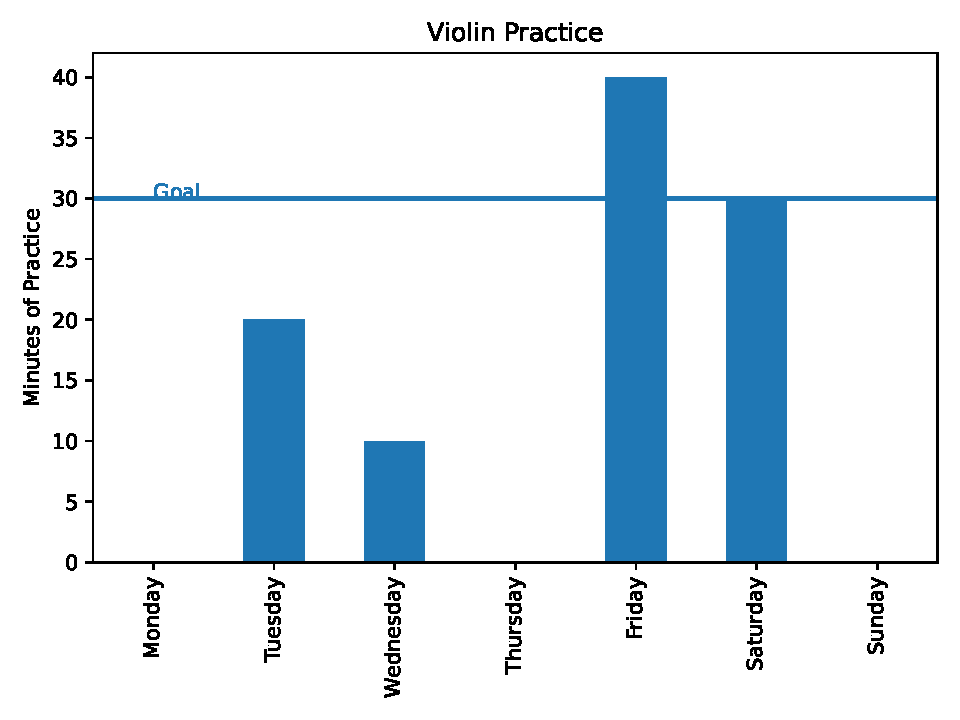
\includegraphics[width = 0.7\textwidth]{figures/poetryplots/violin-bar.pdf}
 \end{center}

This creates a chart that is perfectly fine. But a poet might say, why futz with all the numbers and obfuscate the essential meaning? We only need to know if we hit the goal of 30 minutes or not. This kind of simplification might be more motivating. There's probably some psychology research that supports this, but we'll proceed without deferring to any such authority because those studies so often fail to replicate. Let's create a simple activity calendar of sorts.

%intensity to communicate streaks

\pyfile{violin-cal.py}

 \begin{center}
     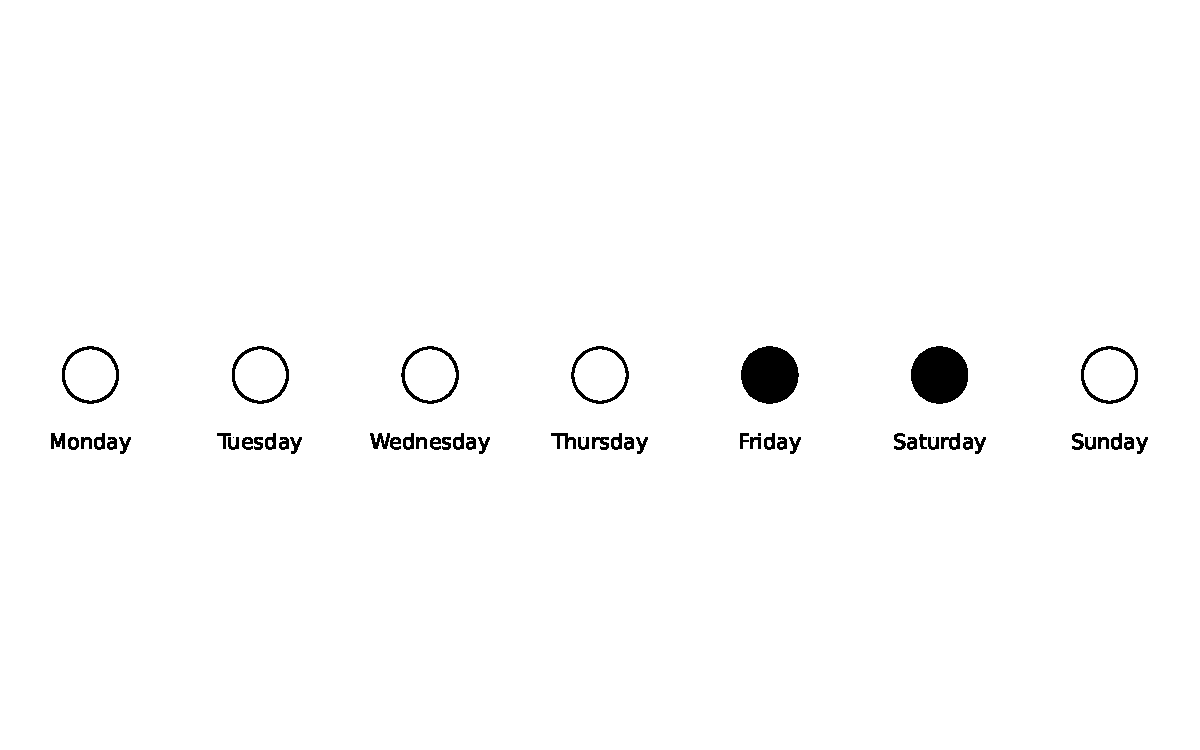
\includegraphics[width = 0.9\textwidth]{figures/poetryplots/violin-cal.pdf}
 \end{center}
 
 You might have in mind ways to spice up this plot even further. Maybe there should be partial credit given to days some with violin practice, but not at least 30 minutes. Perhaps on those days, the circles can be filled with a light gray. The key here is that we're creating a plot that we might think will be more motivating. 
 
 Apps like Duolingo or Peloton gamify the user experience, and part of that is rewarding activity streaks over consecutive days. Let's try to enhance the plot so that streaks stand out. We'll accomplish this by adding a yellow edge color and increasing its weight as a streak continues.
 
\pyfile{violin-streak.py}
 
 \begin{center}
     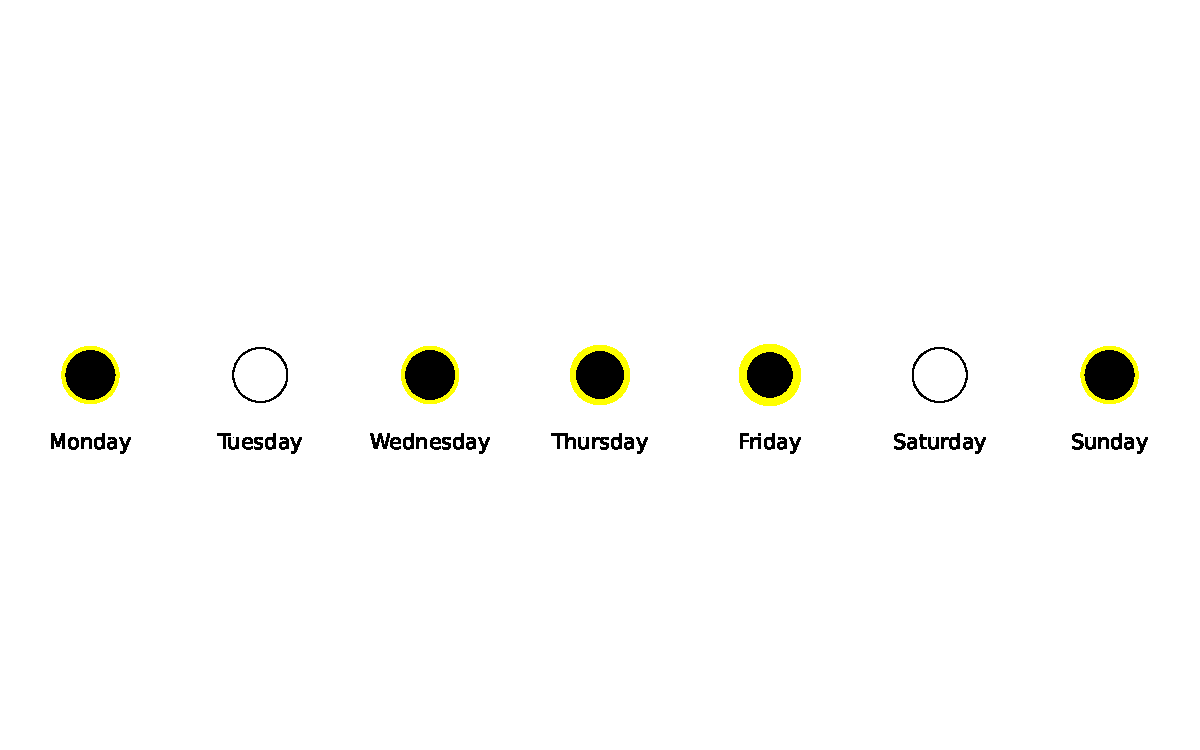
\includegraphics[width = 0.9\textwidth]{figures/poetryplots/violin-streak.pdf}
 \end{center}